\documentclass[10pt]{article}
\usepackage{alltt}
\usepackage[pdftex]{graphicx}
%% \usepackage{graphics}
\usepackage{epsfig}
\usepackage{fullpage}
\usepackage{eso-pic} 
\usepackage{hyperref}
\usepackage{epsfig}
\usepackage{amssymb,amsmath}
\usepackage{listings}
\usepackage{float} 
\usepackage[pdftex]{graphicx}
\usepackage{epstopdf} 
\usepackage[usenames,dvipsnames]{color}
%\usepackage[13pt]{extsizes}
\hypersetup{%
    pdfborder = {0 0 0}
}
% Title Page
\title{\color{Violet}Simple Web}
\author{Anuja Agrawal(CS09B028)\\ Vaibhav Agarwal(CS09B046)}
\lstset {frame=shadowbox, backgroundcolor=\color{darkgray},rulesepcolor=\color{Black}, numbers = left, language = C++, numberstyle=\footnotesize,basicstyle=\normalsize, numbersep=5pt ,morecomment=[l]}
\definecolor{darkgray}{rgb}{0.95,0.95,0.95}



\begin{document}
\maketitle

\section{\color{Violet}Problem Statement}
To design and implement a simple Web .Support for pseudo-HTML with plain ASCII text, links and dialogue capability.

\section{\color{Violet}WorkFlow}
\begin {figure}[ht]
   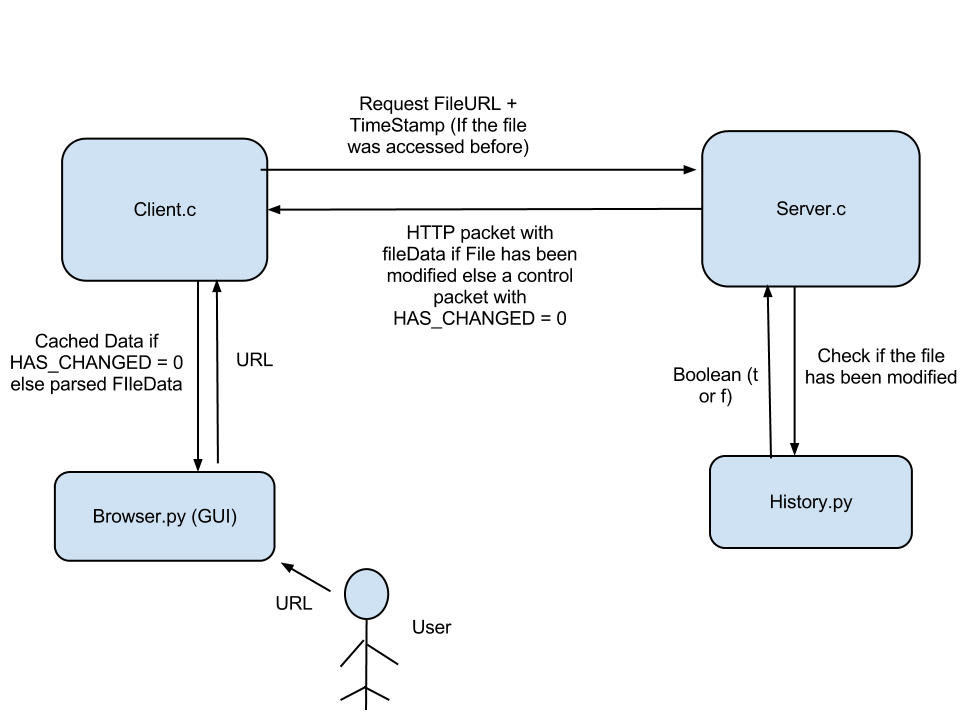
\includegraphics[width=1.0\textwidth]{./SRS.png}
 \end{figure}

\section{\color{Violet}How it works?}
The Simple Web project tries to implement the HTTP protocol using its own markup
language called the markem language. Using a DATAGRAM circuit, we implement a
file transfer protocol. This will help in communication between the user and the client.
The browser as such is limited in it features in that it can only show text , images and
links. As for formatting of text, as of now only color is being proposed as a possible
style option.
For the browser to work, the client will send a request for a file using a certain
format.The server processes the request and sends the reply back to the client in terms
of the specified HTTP protocol. This can be done either by framentation / direct
message passing.This part of the code is written in C. Once we have the file, we scan
the file for text and images.This parsing will be done using Python libraries and then
displayed using Tkinter - another python library.
Some of the assumptions made for the same are :
\begin{itemize}
 \item Any file or image being viewed is not saved in temp, but is instead saved in the
directory for as long as the viewer is in the browser. We could have instead saved
the file in some temporary folder and deleted it after the page has been viewed.But
this will not be implemented here.
\item The basic datagram socket with UDP send / receive will be used to transmit the
message . In addition, since the major criteria is the implementation of the HTTP
protocol, we would limit ourselves to stop-and-wait protocol.
\item The images cannot be created as links in any file. Also the example files must have
a appropriate language.A file with incorrect tags will not be parsed in the right
manner. No type-checking / defaulting will be done in such a case.
\item The browser will be mundane and will not support any sort of keyboard shortcuts.
This is more due to time constraints than any other reason.
\end{itemize}

\subsection{\color{Violet}How to Run : }
\begin{itemize}
 \item  Run the make file, that will create all the necessary executables
\item Run the server by doing a \textbf{./server <portNumber> }
\item Run the browser by doing a \textbf{python sweb.py <portNumberServer> <IPAddressServer>}
\item Enter the fileURL in the dialogBox
\item Once the file is loaded, other queries can be made, by 
\begin{itemize}
 \item Again requesting for a URL in the diaglogBox
  \item Clicking on the links in the current markem page.
\end{itemize}

\end{itemize}
\end{document}          
